\documentclass[main.tex]{subfiles}
\begin{document}
  
  
  \section{Intended Classifications}
  
    The main objective of the project is to provide a classifier that is capable of identifying the type of function that best describes the Data Set that is analysed. This may be more than one function in different segments of the Data Set. Once a function is identified it is conceptually trivial to fit an exact equasion to the data with the use of regression \cite{}. 
    \\\\
    Below is a list of the different classifications that are expected of the software, and the physical significance of them.
    
    \subsection{Points of Interest}  
    \label{sec:POI}
    
    At the core of this project is the identification of \textit{Points of Interest} or POI in Data Sets. A \textit{POI} is the data point at which a sudden change within the Data Set is detected. "Sudden" in the sense that it is not in accordance with the underlying pattern. For example, outliers are data points that were affected by some form of noise, like an insect passing by a visual sensor or a slammed door off-setting a seismometer sensor. As POI can describe impurities in the data they are intended to prompt higher level analysis. They may mark outliers to be simply removed, or a bias in the data that should be corrected for (see \cref{fig:poi:outlier,fig:poi:bias}). 
    \\\\
    The most significant role of POI, however, is to point out interesting features in the data, that might reveal further information about the underlying physical phenomena. To continue the seismometer example from above, certain rumblings in the ground may hint at far away or future earthquakes, and would prompt according warnings. These rumblings would break the silence that underlies the data recorded by this sensor. POI are intended to mark these phenomena for further analysis, either by a human or by more complex computational methods.
    
    \begin{figure}[h]
      \begin{subfigure}{0.48\linewidth}
        \centering
        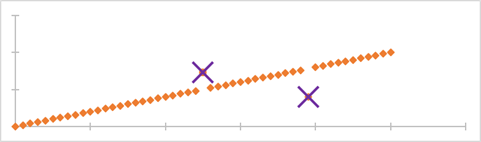
\includegraphics[width=0.9\linewidth]{figures/outlierPOI}
        \caption{Outliers}
        \label{fig:poi:outlier}
      \end{subfigure}
      \begin{subfigure}{0.48\linewidth}
        \centering
        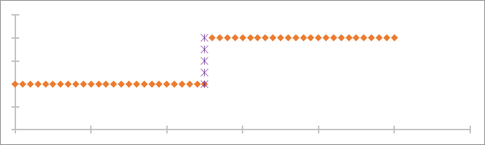
\includegraphics[width=0.9\linewidth]{figures/biasPOI}
        \caption{Bias}
        \label{fig:poi:bias}
      \end{subfigure}
      % leaving blanck lines helps with line-spacing and forces subfigures on separate lines
      
      \begin{subfigure}{0.48\linewidth}
        \centering
        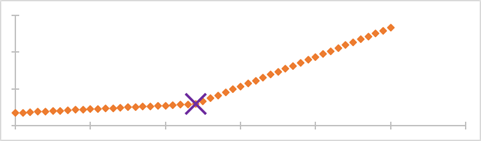
\includegraphics[width=0.9\linewidth]{figures/linearPOI}
        \caption{Change of FFunctionof Same Type}
        \label{fig:poi:linear}
      \end{subfigure}
      \begin{subfigure}{0.48\linewidth}
        \centering
        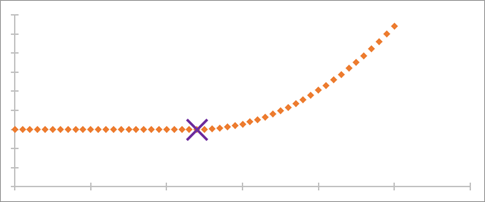
\includegraphics[width=0.9\linewidth]{figures/linSquPOI}
        \caption{Change of Function Type}
        \label{fig:poi:linSqu}
      \end{subfigure}
      \caption{Conceptual examples of different Points of Interest (POI) marked in purple crosses over the underlying data sets in orange. (\subref{fig:poi:outlier}) shows outliers in the data, single data points that are out of place. These types of POI are typically due to noise. (\subref{fig:poi:bias}) shoows a "Bias" in the data, where all data points past the POI are shifted by a constant amount. This is usually a systematic error due to a sensor issue. (\subref{fig:poi:linear}) is an example where the underlying function obviously changes in the POI. This is normally due to a physical change that depends on the phenomena that are being observed. Here only the shape of the function changes, not the type, suggesting that a physical parameter has changed, but not the underlying phenomena. (\subref{fig:poi:linSqu}) on the other hand shows an example where the type of function changes in the POI, suggesting that something has fundamentally changed in the observed phenomena.}
      \label{fig:poi}
    \end{figure}
    
    \Cref{fig:poi} shows some conceptual examples of how POI should be applied. As it demonstrates there are two types of POI, those that mark a physical change and those that mark sensor errors. The latter can be distinguished from the former easily when comparing the functions before and after the POI. Noise does not affect the type of function, or even its shape, so if the difference in function is merely in a constant term or non-existent, within some precision, then the POI can be disreggarded as noise. While this project only aims at producing a classifier, this interpretation of POI into noise or interesting phenomena, and then further interpretation, is the intended future path of the project.
    
    \subsection{Functions}
    
    As this project aims to make use of the derivative to classify data, only functions with characteristic derivatives can be classified. The functions listed here have different characteristics that should allow some degree of certainty when classifying them.
    \paragraph{Polynomials} are of the form $f_{(x)}=\sum_{i=0}^{N} a_i x^i$ such that $i \in \mathbb{N}^\geq$, and represent perhaps the simplest form of functions that should be classified. They are commonly used in the modelling of drag, kinetics, electric current and material properties under stress or temperature changes, among many other applications. 
    \\\\
    In addition to this, a first order polynomial ($a x + b$) is a common component of many other functions, especially when considering $a=1$ and $b=0$, and as such may have considerable influence on these functions as well.
    \paragraph{Exponential} functions are any of the form $f_{(x)}= a A^{g(x)} + b$, where $g_{(x)}$ is a first order polynomial. Any such function is equivalent to $ f{(x)} =  a exp[  Ln(A) g_{(x)}  ] +b $ and should be modelled as such. 
    \\\\
    Exponential functions are common in the physical world, with applications in population growth, radioactive decay, quantum mechanics and more. Most significantly, it is mathematically related to many other functions.
    \paragraph{Rational} functions represent a ratio between polynomials, such that $f_{(x)}=\frac{g_{(x)}}{h_{(x)}}$ and both $g_{(x)}$ and $h_{(x)}$ are polynomial. In its simplest form this is simply $f_{(x)}=\frac{1}{h_{(x)}}$, also written as $f_{(x)}=h_{(x)}^{-1}$. This is commonly used to model the strength of fields as well as other quantities that are based on the distance from a point, due to the \textit{Inverse Square Law} \cite{}. 
    \paragraph{Roots} are an adaptation of polynomials where $i \in \mathbb{Q}^\geq$ is allowed, with the simplest example being $f_{(x)}=\sqrt{x}$. This characteristic may be of use when attempting to classify them. They are less commonly used and of lower priority.
    \paragraph{Allometrics} are functions of the form $f_{(x)}=\sum_{i=0}^{N} a_i x^{b_i} $ where $a_i,b_i \in \mathbb{R}$. They encompass polynomials, roots and rationals. Outside of these subtypes they are quite rare in the physical universe and are of very low priority.
    
    \subsection{What Should Not be Classified}
    
    As stated previously, not all functions may be classified correctly solely based on their derivative. In particular, however, periodic and other trigonometric functions can very easily be classified using a \textit{Fast Fourier Transform} or \textit{FFT} \cite{}.
    \paragraph{Periodic} functions are any function that repeats itself in regular intervals, with the simplest continuous example being the \textit{sine} function of the form $a \sin(b x + c) + d$. Any periodic shape can be approximated to an arbitrary precision with a combination of \textit{sine curves}, even if the shape is discontinuous, like the \textit{square wave}. Hence, these functions are best analysed using the \textit{FFT} instead \cite{}.
    \\\\
    They represent many physical phenomena, as both \textit{oscillations} and \textit{waves} in turn represent many diverse phenomena. These include pendulae, quantum mechanics, fluid dynamics, elastic materials, certain circuits and many more.
    \paragraph{Other Trigonometrics} that are not necessarily periodic include the \textit{hyperbolic function}. As their name suggests, they are a form of \textit{trigonometric function} and are best analysed similarly, making use of \textit{FFT}, despite not being periodic. In a sense they are periodic with an infinite period. 
    
    As FFT analysis has been implemented many times it is not a priority.
    
    \subsection{Combinations of Functions}
    \label{sec:back:combFunc}
    
    Combinations of functions cannot always be extracted correctly. Functions can be combined for example by \textbf{Nesting} of the form $f(g_{(x)})$, such that each function in turn affects the derivative in different ways. With some limitations, it may be possible to remove $f$ by applying its inverse, for example by taking the \textit{natural logarithm} such that $g_{(x)}=Ln\left [ f(g_{(x)})\right ]$ if $f(g_{(x)}) = e^{g(x)}$. However, unless there are reasons to suspect this particular function then all possible inverses must be applied to find the correct one. If the function is nested more than one level the possibilities grow combinatorially. 
    
    % Also show, perhaps with proof, that this would not be any better with machine learning, as the information is basically hidden until it is unppacked.
  
  \section{The Necessity of Machine Learning}
  
    As is typically the case, there are many methods available to tackle the problem at hand. Machine Learning appears to be a particularly common suggestion that is used in a true myriad of applications \cite{}. Here I wish to give an overview of why, in my opinion, machine learning is an unnecessarily complex solution to this somewhat simple problem, and how it will most certainly be applicable in later project stages, making use of information extracted by the methods presented here.
    
    \subsection{The Complexity}
    
    Talk about the unpredictability of learning. By definition ML allows the resulting software to be beyond what the human can predict. Justify this with references and distil into one thought.
    
    \subsection{The Alternative}
    
    This is basically simple physics applied to and integrated in software. It can be based on rigorous mathematics and hence reduce complexity and testing.
    \\\\
    This project is intended to explore an alternative to machine learning approaches, which perhaps could be more or less efficient at the tasks at hand. 
    
    \subsection{Comparable Applications}
    
    \paragraph{Edge Detection} also makes use of derivative \cite{}. Minor differences maybe? \\
    Very similar example of purely mathematical analysis that then informs higher level and ML analysis.
    
    \subsection{Machine Learning in the Future}
    
    Have ML make use of this information and classify on a higher level. This way it can make use of rigorous mathematics, but fill out the gaps that are normally filled by human expertise. Additionally this approach reduces the need to teach the machine, and hence eases the way for good ML \cite{}.
    
\end{document}